
\documentclass[11pt,twoside]{article}

\usepackage[utf8]{inputenc}
\usepackage{graphicx}
\usepackage{amsmath}
\usepackage{amssymb}
\usepackage{url}
\usepackage{graphics}
\usepackage{wasysym}
\usepackage{enumitem}
\usepackage[english,portuges]{babel}
\usepackage{color}
\usepackage[usenames,dvipsnames]{xcolor}



\begin{document}

%*********************************************************************** TITULO

\section*{
    Esquema de interpolação alternativo para a reso\-lução numérica de
problemas de difusão com convecção usando o método dos volumes finitos
}

\vspace{10pt}


%************************************************************************* AUTORES
Luís J.M. Amoreira$^{1}$%, Nome Sobrenome$^{1,2}$, Nome Sobrenome$^{1,2}$

\vspace{10pt}


%************************************************************************** MORADA

{
\center

    \footnotesize

$^{1}$ Departamento de Física e CMAST, Universidade da Beira Interior, Covilhã, 
Portugal \\
E-mail: amoreira@ubi.pt

%\vspace{3pt}
%
%$^{2}$ Endereço 2, Portugal \\
%Email:  email2@email.pt
%
%\vspace{3pt}
%
%$^{3}$ Endereço 1, Portugal
%
}

\vspace{25pt}

%%%%%%%%%%%%%%%%%%%%%%%%%%%%%%%%%%%%%%%%%% RESUMO


{\setlength{\parindent}{30pt}%

\small%
\section*{Resumo}
\smallskip
%%%%%%%%%%%%%%%%
%Corpo do resumo (aprox. 200 palavras)
Neste trabalho é proposto um esquema de discretização alternativo para a
resolução de problemas de difusão com convecção baseado no esquema de diferenças
centrais mas com coeficientes de interpolação que dependem da velocidade
convectiva.

É feita uma análise comparativa do esquema proposto com esquemas tradicionais
(diferenças centrais, \emph{upwind}, híbrido), em termos da estabilidade, da
exatidão e da taxa de convergência. O problema usado para a comparação é o da
difusão estacionária undimensional num fluido imcompressível em escoamento com
velocidade constante, para o qual existem soluções analíticas.

Verifica-se que o esquema proposto é estável mesmo em problemas com convecção
intensa e que produz, em geral, resultados mais aproximados da solução analítica
dos que os obtidos com os restantes esquemas considerados. Como o esquema de
difrerenças centrais, o esquema proposto é de segunda ordem em malhas homogéneas
centradas.

\vspace{15pt}





%%%%%%%%%%%%%%%%%%%%%%%%%%%%%%%%%%%%%%%%%%%    SECTIONS  %%%%%
\section{Introdução}
%Corpo de texto regular, com referencias do estilo [1] e [2, 3]. as referências
%devem ser introduzidas manualmente. O estilo das referências é definido pelos
%editores.
A conservação em regime estacionário e unidimensional de uma propriedade
extensiva de um meio com densidade $\rho$ que se move com velocidade $v$
traduz-se pela equação diferencial [REFS]
\begin{equation}
    S(x) = \frac{dj_d}{dx}+\frac{dj_c}{dx}.\label{eq:dif}
\end{equation}
Nesta expressão, $S(x)$ é a densidade de fonte dessa propriedade e $j_d$ e $j_c$
representam respetivamente as densidades de fluxo difusivo e convectivo da
propriedade, dadas por
\begin{align}
    j_d&=-\Gamma\frac{d\rho\phi}{dx}&
    j_c&=\rho\phi v,
\end{align}
onde $\phi$ é a propriedade por unidade de massa (a sua densidade espacial
é, portanto, $\rho\phi$) e $\Gamma$ o coeficiente de difusão.

Numa resolução da eq.\eqref{eq:dif} com o método dos volumes finitos, define-se
uma partição do domínio de integração num conjuto de subdomínios (chamados
\emph{volumes de controle,} VC), constituindo uma \emph{malha de discretização}
como a ilustrada na Figura~\ref{fig:1}.
\begin{figure}[!h]
    \begin{center}
        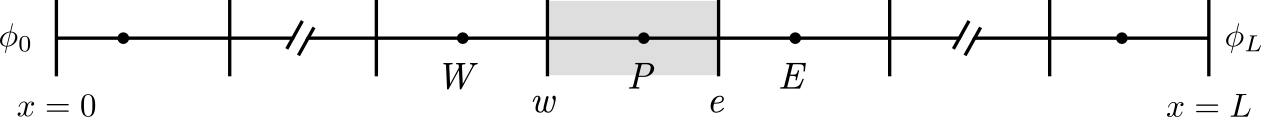
\includegraphics{figs/f10.png}
    \end{center}
    \caption{Partição do domínio de integração num conjunto de volumes de
    controle.\label{fig:1}}
\end{figure}
Integrando-se a equação diferencial em cada um destes subintervalos obtém-se um
sistema de equações algébricas, em número igual ao do dos VC considerados, que
relacionam os fluxos difusivo e convectivo da propriedade através das fronteiras
que separam os VC.  Por exemplo, para a célula destacada na Figura~\ref{fig:1}
resulta:
\begin{equation}
    (\rho v\phi)_e- (\rho v\phi)_w =
    \left(\Gamma \frac{d\phi}{dx}\right)_e-
    \left(\Gamma \frac{d\phi}{dx}\right)_w+S_P\delta x.\label{eq:1}
\end{equation}
Note-se que, num escoamento estacionário unidimensional, a equação da
continuidade garante que o produto $F=\rho v$ é homogéneo.

Neste contexto, um \emph{esquema de discretização} é apenas um procedimento para
estimar os valores dos fluxos nas faces dos VC como funções dos valores dos
campos $\phi$ nos pontos ($W$, $P$, $E$, etc.)

\subsection{Esquemas de discretização tradicionais}
\begin{enumerate}
    \item Esquema de diferenças centrais (CDS)\\
No chamado \emph{esquema de diferenças centrais,} os valores dos termos
convectivos [no lado esquerdo da eq.~\eqref{eq:1}] nas faces dos VC são
estimados por interpolação linear a partir dos valores de $\phi$ nos pontos
nodais dos dois VC que partilham essa face. Isto é, fazem-se na eq.~\eqref{eq:1}
as substituições\footnote{Estas fórmulas são válidas apenas para malhas
    homogéneas e centradas, em que as faces dos VC se encontram nos pontos
    médios entre os pontos nodais. A generalização para os restantes casos é
    óbvia}:
\begin{align}
    \phi_e&= \frac{1}{2}(\phi_P+\phi_E)&
    \phi_w&= \frac{1}{2}(\phi_W+\phi_P),\label{eq:2}
\end{align}
Por seu turno, as derivadas nos termos difusivos [no lado direito da
eq.~\eqref{eq:1}] são avaliadas com a fórmula de derivação numérica central, ou
seja, através das expressões
\begin{align}
    \left(\frac{d\phi}{dx}\right)_e&=
    \frac{\phi_E-\phi_P}{\delta x}&
    \left(\frac{d\phi}{dx}\right)_w&=
    \frac{\phi_P-\phi_W}{\delta x}.
\end{align}
O CDS é um esquema simples e, quando aplicado em malhas homogéneas e centradas,
constitui um método de segunda ordem (o erro das soluções é proporcional ao
quadrado do passo de discretização). No entanto, este esquema produz soluções
instáveis quando o transporte convectivo domina o difusivo.  A importância
relativa dos fluxos convectivo e difusivo é normalmente estimada pelo valor do
chamado \emph{número de Peclet}, igual à razão entre os coeficientes do campo
$\phi$ nas expressões dos dois fluxos:
\begin{equation}
    P=\frac{\rho v}{\Gamma}\delta x
\end{equation}
Verifica-se que as soluções obtidas com o CDS são instáveis para\footnote{Este
    valor numérico concreto está relacionado com os
    coeficientes de interpolação na eq.~\eqref{eq:2}. Em malhas não homogéneas
ou não centradas, outros valores se aplicam.}
$P\gtrsim2$.
Assim, a análise de situações com escoamento significativo só pode ser feita
recorrendo a malhas apertadas.

\item Esquema de diferenças \emph{upwind} (UWS)\\
As soluções CDS têm problemas de estabilidade porque, na expressão adotada para
o fluxo convectivo nas faces dos VC é dada igual importância aos  alores de
$\phi$ nos pontos nodais dos dois VC que partilham essa face. Ora,
intuitivamente, parece recomendável dar maior importância ao valor de $\phi$ no
VC que se situa \emph{a montante}, relativamente ao sentido do escoamento.\\
%
O esquema de diferenças \emph{upwind} adota esta recomendação de forma o mais
radical possível: nos termos convectivos, toma-se para valor do campo $\phi$
numa dada face o valor que ele apresenta no ponto nodal do VC a montante, isto
é, fazem-se no lado esquerdo da eq.~\eqref{eq:1} as substituições
\begin{align}
    \phi_e&=
    \begin{cases}
        \phi_P,&P>0\\
        \phi_E,&P<0
    \end{cases}&
    \phi_w&=
    \begin{cases}
        \phi_W,&P>0\\
        \phi_P,&P<0
    \end{cases}
\end{align}
Os termos difusivos, por seu turno, são tratados tal como no CDS.\\
%
O UWS é estável independentemente da velocidade do escoamento, mas é pouco
exato, especiamente (e como era expectável) para escoamentos muito lentos.
Trata-se de um esquema de primeira ordem, ou seja, a sua convergência é bastante
mais lenta do que a do CDS.

\item {Esquema híbrido (HYB)}\\
No esquema híbrido tenta-se reunir as qualidades dos dois esquemas anteriores.
Quando o escoamento é lento (mais concretamente, quando $|P|<2$), este esquema
consiste no CDS; pelo contrário, quando o escoamento é rápido ($|P|>2$) adota-se
o UWS, e desprezam-se ainda os fluxos difusivos.\\
%
O esquema híbrido é também estável, e bastante exato tanto para escoamentos
muito lentos como para escoamentos muito rápidos, mas menos para regimes
intermédios. Uma outra desvantagem deste esquema ocorre em situações não
estacionárias: nessas situações podem gerar-se descontinuidades espúrias nas
soluções por ocorrer uma mudança no regime seguido pelo esquema.
\end{enumerate}

\section{Esquema de ajuste contínuo}

\section{Resultados}
\section{Conclusões}
%%%%%%%%%%%%%%%%%%%%%%%%%%% TABELA
%\begin{table}[!h]
%\caption{Legenda da tabela.}
%
%\end{table}



%%%%%%%%%%%%%%%%%%%%%%%%%%% FIGURA
%\begin{figure}[!h]
%\centering
%\includegraphics[scale=0.95]{fig_1.pdf}
%\caption{Legenda da figura.}
%\end{figure}








%%%%%%%%%%%%%%%%%%%%%%%%%%%%%%%%%%%%%%%%%%%    SECTION  %%%%%
\section{Conclusões}

\begin{itemize}

\item Conclusão 1

\item Conclusão 2


\end{itemize}




%%%%%%%%%%%%%%%%%%%%%%%%%%%%%%%%%%%
%%
%%                 AKNOWLEDGMENTS & BIBLIOGRAPHY
%%
%%%%%%%%%%%%%%%%%%%%%%%%%%%%%%%%%%%

{\footnotesize%


%%%%%%%%%%%%%%%%%%%%%%%%%%%%%%%%%%%%%%%%%%%    AGRADECIMENTOS  %%%%%
%\section*{Agradecimentos}
% Text







%%%%%%%%%%%%%%%%%%%%%%%%%%%%%%%%%%%%%%%%%%%    REFERÊNCIAS  %%%%%
\section*{Referências}
\vspace{5pt}

\begin{enumerate}[label={[\arabic*]}]

\item	Laugksch R., Scientific Literacy: A Conceptual Overview Science Education, 84, 71-94, 2000.

\item	Driver, R., Young people's images of science, Open University Press (Buckingham and Bristol, PA) 1996.

\item	Lopes J.B., Pinto J., Silva, A. Situação formativa: um instrumento de gestão do currículo capaz de
promover literacia científica. Enseñanza de las Ciencias, Número Extra VIII Congreso Internacional sobre
Investigación en Didáctica de las Ciencias, Barcelona, pp. 1624-1629 2009.



\end{enumerate}

}


\end{document}
